\documentclass{beamer}
\mode<presentation>
{
  \usetheme{default}      % or try Darmstadt, Madrid, Warsaw, ...
  \usecolortheme{default} % or try albatross, beaver, crane, ...
  \usefonttheme{default}  % or try serif, structurebold, ...
  \setbeamertemplate{navigation symbols}{}
  \setbeamertemplate{caption}[numbered]
}

\usepackage[spanish]{babel}
\usepackage[utf8x]{inputenc}
%\usepackage{hyperref}
%\usepackage[latin1]{inputenc}
%\usepackage{times}
%\usepackage[T1]{fontenc}

\title[Clase 1]{Procesamiento de bases de datos con STATA}
\subtitle{Clase 1}
\author{Claudia Vazquez}
\date[]{\texttt{clauvazqu@gmail.com}\\Centro REDES}
\pgfdeclareimage[height=0.4cm]{university-logo}{logo-redes}
\logo{\pgfuseimage{university-logo}}

\begin{document}
\begin{frame}
  \titlepage
\end{frame}

\begin{frame}{Contenido}
  \tableofcontents
 \end{frame}

%\part{Tutorial}
%\frame{\partpage}



\begin{frame}{Modalidad del curso I}
\begin{itemize}
\item El objetivo de este curso es aprender el manejo básico del paquete estadístico STATA.
\item El alumno deberá tener instalado el programa.  
\item El curso se compone de cuatro módulos de dos clases cada uno, con una duración total de 8 semanas.
\item Cada clase equivale aproximadamente a una clase presencial de tres horas, pero si el alumno no tiene experiencia con el programa conviene que avance despacio y le dedique más tiempo.
 \item El curso no tiene horarios preestablecidos: usted puede leer las clases y realizar la ejercitación en el momento que más le convenga.
\end{itemize}
\end{frame} 

\section{Presentación del curso}
\subsection{Aspectos organizativos}
 
 \begin{frame}{Modalidad del curso II}
\begin{itemize}
\item Todos los martes se subirá una clase a la plataforma virtual y el ejercicio práctico correspondiente, que deberá ser entregado en el lapso de diez días corridos (el viernes siguiente).
\item Se recomienda \textbf{siempre} tener STATA abierto mientras se leen las clases, de forma de ir practicando los comandos que se aprenden.
\item El foro de discusión estará disponible en todo momento para realizar consultas e intercambios sobre las clases. 
\item Se recomienda visitar y participar del foro ya que enriquese la experiencia del curso. 
\end{itemize}
\end{frame}



\begin{frame}{Tipografía del curso}
En el curso utilizamos algunas convenciones tipográficas para indicar cómo se utilizan las palabras: 
\begin{itemize}
\item Los  comandos se escriben en \texttt{esta tipografía} y el usuario debe tipearlos en la línea de comandos siempre en letras minúsculas.
\item Cuando se pega una imagen de la ventana de resultados de STATA, la línea de comandos comienza con un punto, que \textbf{no} debe escribirse.  
\item Algunas palabras aparecen en \textit{cursiva} para indicar que no deben tipearse tal cual sino sustituirse por otra: por ejemplo, los nombres de variables (\textit{varname}) o archivos (\textit{filename}). 
\end{itemize}
\medskip
Ejemplo de la tipografía:\\
. \texttt{list \textit{varname}}
\end{frame}

\subsection{Presentación de STATA}


\begin{frame}{Características}
 \begin{itemize}
\item STATA es un paquete estadístico para la gestión y el análisis de bases de datos y la realización de gráficos. 
\item Se puede utilizar a mediante la interfaz gráfica de usuario (GUI, por sus siglas en inglés), haciendo \textit{click} con el mouse sobre los íconos, o mediante comandos.
\item Si bien la GUI provee una interfaz sencilla para quienes recién comienzan a utilizar el programa, el lenguaje de comandos permite comunicar a STATA ideas más complejas y de una manera mucho más rápida.
\item En este curso aprenderemos a comunicarnos con STATA mediante el lenguaje de comandos.
\end{itemize}
\end{frame}

\begin{frame}{Otras características}
 \begin{itemize}
\item STATA es programable, es decir, admite la creación de nuevos comandos por parte de los usuarios (que suelen resultar muy útiles). 
\item SSC (Statistical Software Components) es el principal sitio de Internet para bajar comandos escritos por usuarios. Podemos encontrar, instalar y desinstalar cualquier módulo de SSC desde STATA con el comando \texttt{ssc}. 
\item STATA tiene un sistema de ayuda muy completo y es importante consultarlo permanentemente. La ayuda puede buscarse por tema o por comando. 
\item Cuando escribimos \texttt{help} seguido por el nombre de un comando accedemos al archivo que lo describe y explicita su sintaxis. 
\end{itemize}
\end{frame}


\begin{frame}[allowframebreaks]{Memoria}
\begin{itemize}
\item STATA trabaja de una manera particular: toda la base de datos a utilizar es almacenada en la memoria RAM.
\item La ventaja es que la ejecución de los comandos es muy rápida. La desventaja, que el tamaño de las bases que pueden procesarse se encuentra limitado por la cantidad de memoria del equipo.
\item En la versión 11 y anteriores STATA comienza la sesión con una cantidad de memoria asignada por defecto (10M). 
\item Si la base que queremos utilizar es más grande, debemos ampliarla (a los efectos de este curso probablemente no sea necesario). 
\item Para ampliar la memoria debemos utilizar el comando \texttt{set memory} seguido por la cantidad de bytes (b), kilobytes (k), megabytes (m) o gigabytes (g) que queramos asignar: \\
. \texttt{set memory 50m}
\item La memoria que se le asigna a STATA se le quita al sistema operativo, por lo que se harán más lentas las tareas que se ejecuten simultáneamente (no la amplíen si no lo necesitan!).
\item Para que STATA nos permita modificar la memoria asignada es necesario que no haya una base ya cargada en memoria: si queremos ampliar la memoria con una base cargada nos da el siguiente error:\\\smallskip
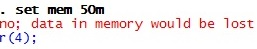
\includegraphics[height=1cm]{mem.jpg}
\item Para poder hacerlo debemos quitar la base en memoria con el comando \texttt{clear}.
\item A partir de STATA 12 el ajuste de memoria es automático.
\item Algo a tener en cuenta si trabajamos con bases muy grandes es que Windows 32 bits no permite asignarle a ninguna aplicación más de 1GB de memoria, independientemente de cuánto tenga la PC.
\end{itemize}
\end{frame}

\begin{frame}{Diferentes versiones de STATA}
\begin{itemize}
\item \textbf{MP}: Versión diseñada especialmente para procesadores dual-core o multicore.
\item \textbf{SE}: Al igual que la \textbf{MP}, puede trabajar con bases de hasta $32.767$ variables. 
\item \textbf{IC}: Puede trabajar con bases de hasta $2.047$ variables. 
\end{itemize}
En todas estas versiones la cantidad de observaciones está limitada solo por la memoria RAM.
\begin{itemize}
\item \textbf{Small STATA}: Versión para bases pequeñas, limitada a 99 variables y $1.200$ observaciones.
\item Todas las versiones están disponibles para las plataformas:
\begin{itemize}
\item Windows (32-bits), Windows (64-bits)
\item Mac (32-bit Intel), Mac (64.bit Intel), Mac (Power PC)
\item Linux (32-bit), Linux (64-bit x86-64), Linux (64-bit Itanium)
\end{itemize}
\item Para saber cuál tenemos instalada usamos el comando \texttt{about}
\end{itemize}
\end{frame}



\begin{frame}{Base de datos en STATA}
\begin{itemize}
\item El contenedor de datos en STATA se denomina \textit{dataset}
\item Un \textit{dataset} es una de tabla de doble entrada donde las columnas se denominan \textbf{variables} y las filas \textbf{observaciones}\\
\begin{center}
\smallskip
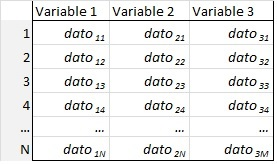
\includegraphics[height=2.3 cm]{base.jpg}
\smallskip
\end{center}
\item Como veremos más adelante, en cada celda pueden guardarse datos de diferente tipo: números, fechas, palabras. El tipo de dato es el mismo para las observaciones de una misma variable.
\end{itemize}
\end{frame}



\begin{frame}{Interfaz de ventanas}
Cuando abrimos STATA vemos las principales ventanas que conforman la interfaz:
\begin{itemize}
\item \textbf{Variables}: muestra las variables de la base de datos actualmente cargada en la memoria.
\item  \textbf{Command}: es la ventana donde el usuario introduce los comandos.
\item \textbf{Results}: muestra los resultados obtenidos por la aplicación de los comandos.
\item \textbf{Review}: muestra el historial de comandos utilizados recientemente.
\end{itemize}
\end{frame}

\begin{frame}{Interfaz de ventanas}
\centerline{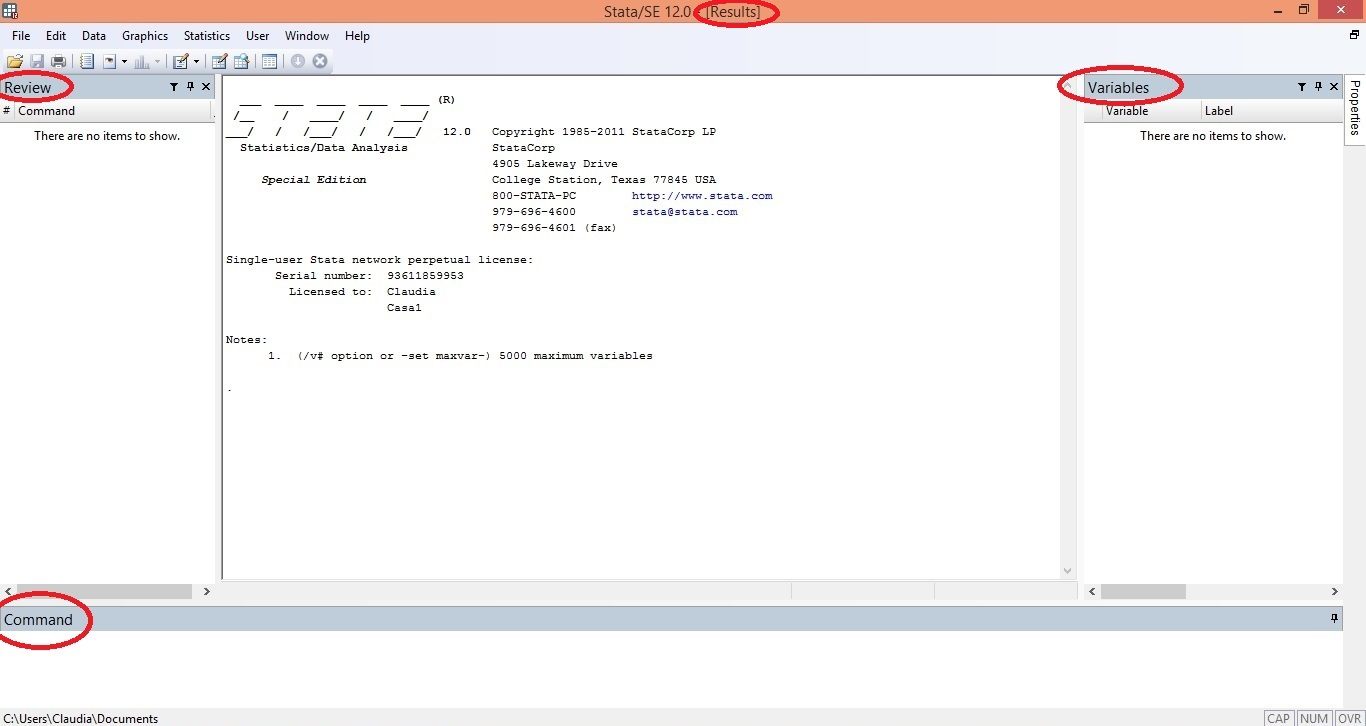
\includegraphics[height=6.5cm]{Ventanas.jpg}}
\end{frame}

\begin{frame}{Interfaz de ventanas}
\begin{itemize}
\item En la figura anterior, la ventana \textbf{Variables} está vacía porque aún no hemos cargado ninguna base de datos en la memoria.
\item Como tampoco hemos ingresado ningún comando, también las ventanas \textbf{Review} y \textbf{Results} están vacías.
\item Ahora vamos a cargar una base: tipeamos en la ventana \textbf{Command} la siguiente instrucción (y le damos enter): \texttt{sysuse} auto.dta 
\item Observamos que en la ventana \textbf{Variables} aparece el listado de variables que contiene la base ``auto''.
\item Además, en la ventana \textbf{Review} quedó almacenada la instrucción tal cual la tipeamos.
\end{itemize}
\end{frame}

\begin{frame}{Interfaz de ventanas}
\centerline{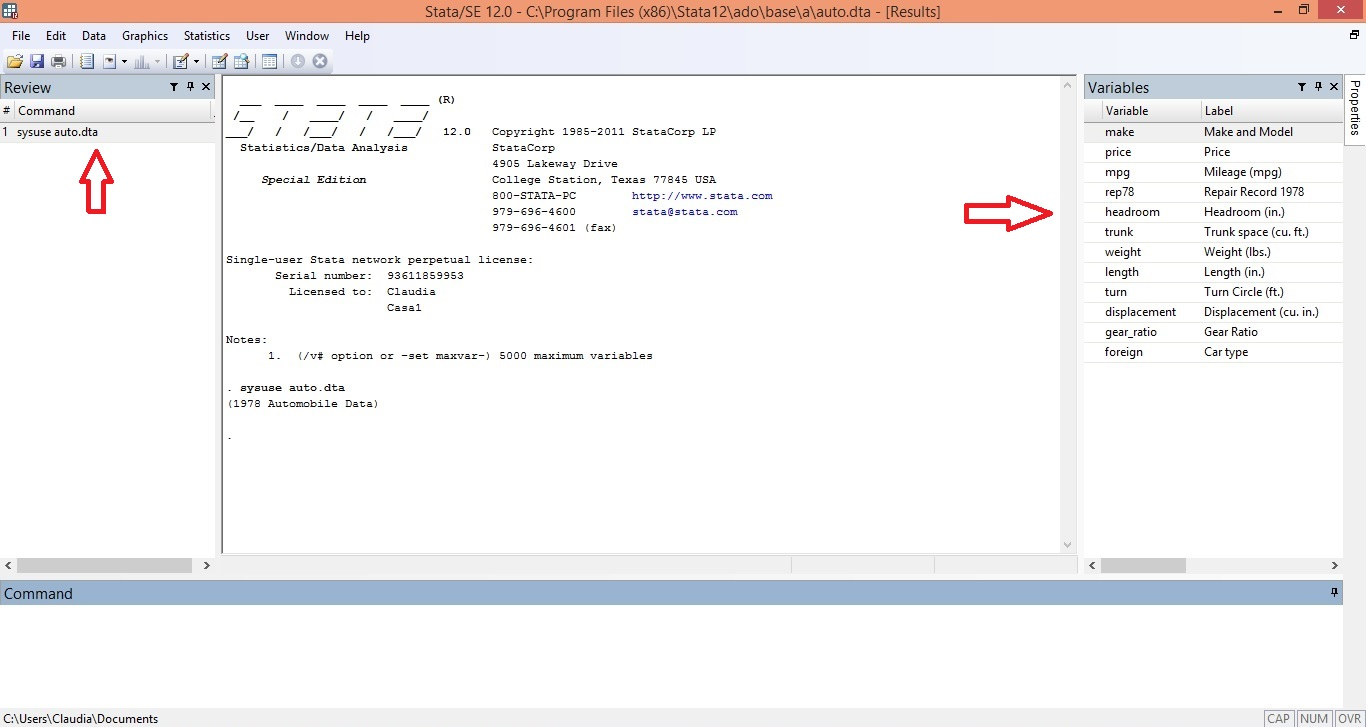
\includegraphics[height=6.5cm]{Ventanas1.jpg}}
\end{frame}


\begin{frame}{Bases de datos utilizadas para practicar}
\begin{itemize}
\item La base auto.dta es un archivo que viene en el directorio oficial de STATA y es utilizado frecuentemente como ejemplo en la ayuda. 
\item Se trata de una base de datos que contiene información sobre el precio, kilometraje, marca y otras características de 74 automóviles.
\item Utilizamos el comando \texttt{sysuse} porque la base viene en el directorio oficial de STATA. Cuando carguemos datos propios que no estén en el directorio de STATA utilizaremos el comando \texttt{use}.
\item ``.dta'' es la extensión del formato de bases de datos de STATA (si no la hubiésemos especificado la habría tomado por defecto). 
\end{itemize}
\end{frame}

\begin{frame}{Bases de datos utilizadas para practicar}
\begin{itemize}
\item La base de autos no es la única que viene en el directorio de STATA. Hay más bases de práctica, como por ejemplo: 
\smallskip
{\small
\begin{center}
\begin{tabular}{p{3cm} p{5cm}} \hline
\texttt{bplong.dta}& Datos sobre presión sanguínea\\
\texttt{cancer.dta} & Datos de un ensayo clínico\\
\texttt{census.dta}& Datos del censo de EEUU\\
\texttt{citytemp.dta}& Datos sobre clima\\
\texttt{educ99gdp.dta}& Datos sobre educación y PBI\\
\texttt{lifeexp.dta}& Datos de esperanza de vida\\\hline
\end{tabular}
\end{center}}
\smallskip
\item Todas se cargan con el comando \texttt{sysuse} más el nombre.
\item Existen otras bases disponibles en Internet para descargar o utilizar directamente con el comando \texttt{webuse}: \url{www.stata-press.com/data/}
\end{itemize}
\end{frame}

\section{Algunos comandos básicos}
\subsection{Describe}
\begin{frame}{Describe} 
\begin{itemize}
\item El comando \texttt{describe} presenta información básica sobre la base de datos en memoria como:
\begin{enumerate}
\item Cantidad de observaciones  
\item Cantidad de variables  
\item Tamaño de la base
\item Tipo de dato de cada variable
\item Si la base está ordenada por alguna/s variable/s
\item Etiquetas de las variables, si existen 
\item Etiquedas de los valores de una variable, si existen
\end{enumerate}
\item Más adelante veremos en detalle qué significan 4 y 5. 
\end{itemize}
\end{frame}

\begin{frame}{Describe}
\centerline{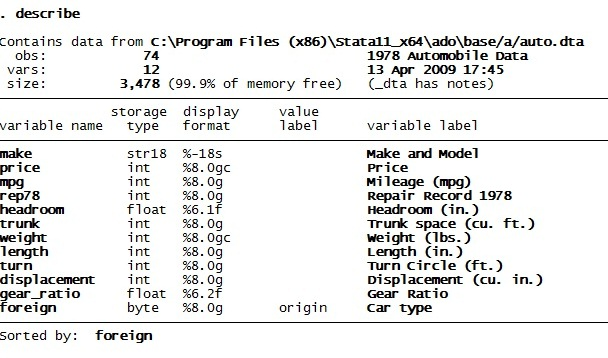
\includegraphics[height=6.5cm]{Describe1.jpg}}
\end{frame}


\begin{frame}{Describe}
En la tabla anterior vemos:
\begin{itemize}
\item Que la base de autos contiene 74 observaciones y 12 variables.
\item Que las variables tienen una etiqueda que las describe (``variable label'').
\item Que solo la variable ``foreign'' tiene una etiqueda para los valores (ver ``origin'' en ``value label'').
\item Que la variable ``make'' es una variable \textit{string}, que quiere decir que es no numérica (ver ``str18'' en ``storage type''). 
\item Que la base está ordenada por la variable ``foreign'' (ver ``sorted by'' al final de la tabla).
\end{itemize}
\end{frame}

\subsection{Browse y Edit}
\begin{frame}{Browse y Edit}
\begin{itemize}
\item Ambos comandos permiten visualizar la estructura del \textit{dataset} (variables en columnas y observaciones en filas).
\item La diferencia es que mientras que \texttt{edit} permite ingresar nuevos datos y editar los existentes, \texttt{browse} solo permite visualizar la base sin poder editarla -es útil cuando queremos ver la estructura de los datos sin temor a introducir cambios no deseados.
\item Cuando ingresamos el comando \texttt{browse} se abre una nueva ventana con el \textit{dataset} y podemos ver el valor de cada variable para cada observación de la base como si fuera una hoja de cálculo (ver figura).
\end{itemize}
\end{frame} 

\begin{frame}{Browse y Edit}
\centerline{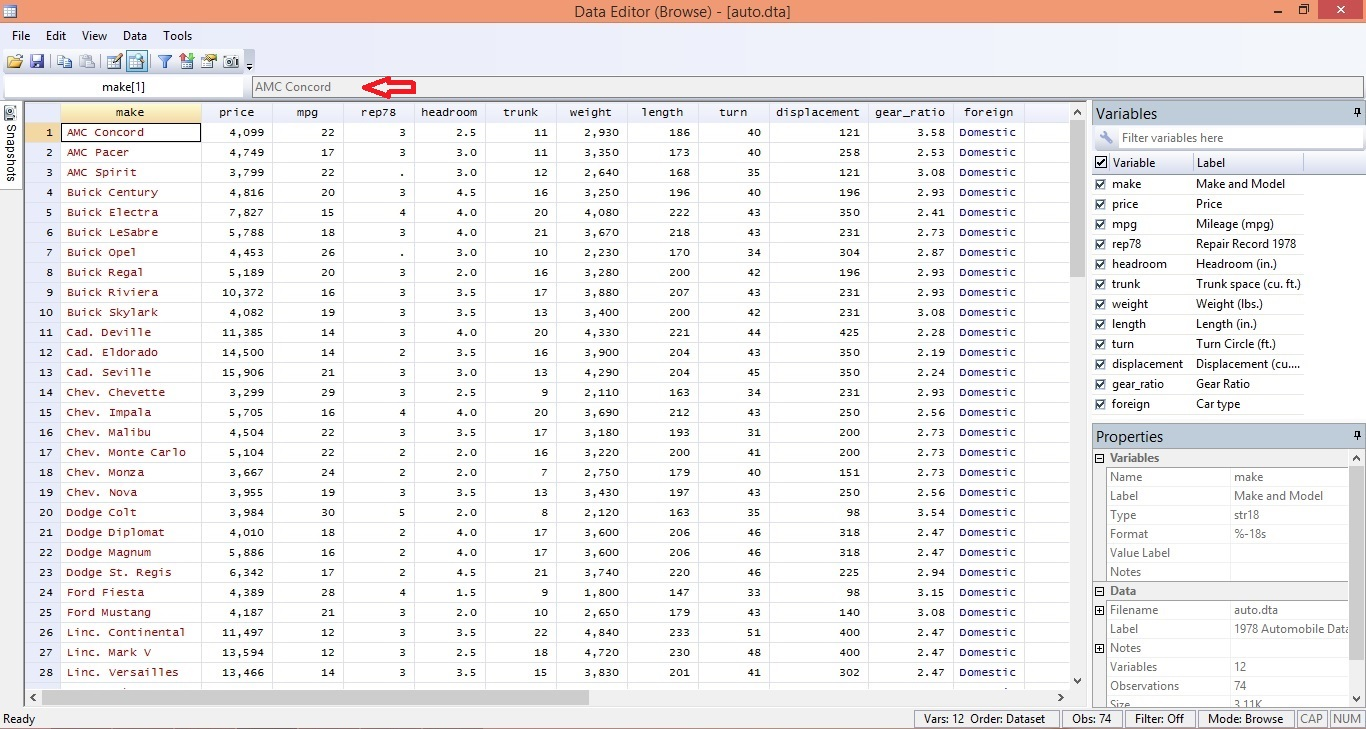
\includegraphics[height=6.5cm]{browse.jpg}}
\end{frame}


\begin{frame}{Browse y Edit}
\begin{itemize}
\item Si desde la pantalla del browse nos paramos sobre alguna de las observaciones de la variable ``foreign'' vemos que, mientras que en la celda dice ``Domestic'' o ``Foreign'', en la parte superior señalada por la flecha se ven ceros o unos. 
\item Esto es porque ``foreign'' es una variable numérica dicotómica a la que se le ha asignado una etiqueta de valores: cero corresponde a ``Domestic'' y uno a ``Foreign''. 
\item Más allá de las etiquetas, la variabe vale cero o uno.
\item Aunque en los ``outputs'' de STATA (tablas, etc.) aparecen las etiquetas, cuando queramos hacer referencia a los valores en la línea de comandos escribiremos $0$ o $1$.
\end{itemize}
\end{frame}

\subsection{Etiquetas}
\begin{frame}{Etiquetas}
\begin{itemize}
\item Es muy útil usar etiquetas. Se pueden asignar etiquetas a:
\begin{itemize}
\item Una base de datos
\item Una variable
\item A los valores que toma una variable  
\end{itemize}
% \item En la base de autos todas las variables tienen una etiqueta.
% \item Más adelante veremos cómo asignar etiquetas. 
% \item Es importante notar que, aunque la variable tenga una etiqueta en sus valores, STATA la sigue considerando una variable numérica.
% \item Por ejemplo, la varaible ``foreign'' toma valores $0$ y $1$, que están asociados respectivamente a las etiquetas ``Domestic'' y ``Foreign''.
\item Los comandos son, respectivamente:
\begin{itemize}
\item \texttt{label data} \textit{"label"}
\item \texttt{label variable} \textit{varname} \textit{"label"}
\item \texttt{label values} \textit{varname} \textit{"lblname"} 
\end{itemize}
\item En el último caso, primero debemos definir el mapeo (``\textit{lblname}'') con el comando \texttt{label define}. 
\item Una vez que creamos la etiqueta, podemos asignarla a los valores de alguna/s variable/s.
\end{itemize}
\end{frame}

\begin{frame}[allowframebreaks]{Etiquetas}
\begin{itemize}
\item Por ejemplo, supongamos que queremos: 
\end{itemize}
\begin{enumerate}
\item Asignarle la etiqueta ``Base de datos de autos para practicar'' al archivo auto.dta. 
\item A la variable ``make'' queremos asignarle la etiqueta ``marca del auto''. 
\item A los valores que toma la variable ``rep78'' (1 a 5) queremos asignarle una etiqueta (que llamaremos ``estado'') que describa el estado del auto en función de cuántas veces fue reparado. 
\end{enumerate}
Ingresamos los siguientes comandos secuencialmente:\\
\medskip
\begin{tabular}{|p{11cm}|}
\hline
{\footnotesize \texttt{label data} ``Base de datos de autos para practicar''}\\
{\footnotesize \texttt{label variable} make ``marca del auto''}\\
{\footnotesize \texttt{label define} estado 1 ``excelente'' 2 ``bueno'' 3 ``medio'' 4 ``regular'' 5 ``malo''}\\
{\footnotesize \texttt{label values} rep78 estado}\\
\hline
\end{tabular}
\begin{itemize}
\item Volvemos a hacer un \texttt{describe} de la base y vemos los cambios.
\item Para ver las etiquetas en los valores de ``rep78'' podemos hacer un \texttt{browse} de la base.
\item Podemos volver a la base original conel comando \texttt{sysuse auto.dta, clear}
\end{itemize} 
\centerline{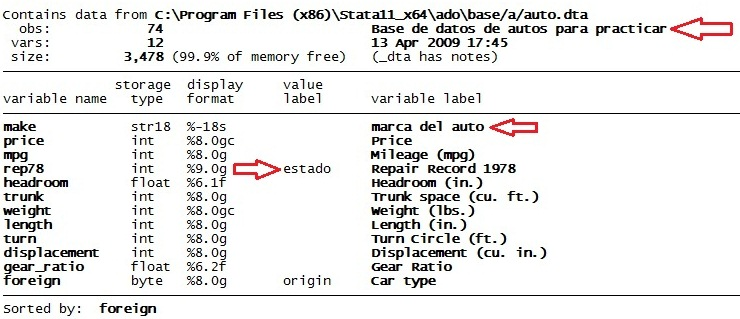
\includegraphics[height=5cm]{label.jpg}}
{\footnotesize Observamos los cambios realizados en las etiquetas.}\\
\centerline{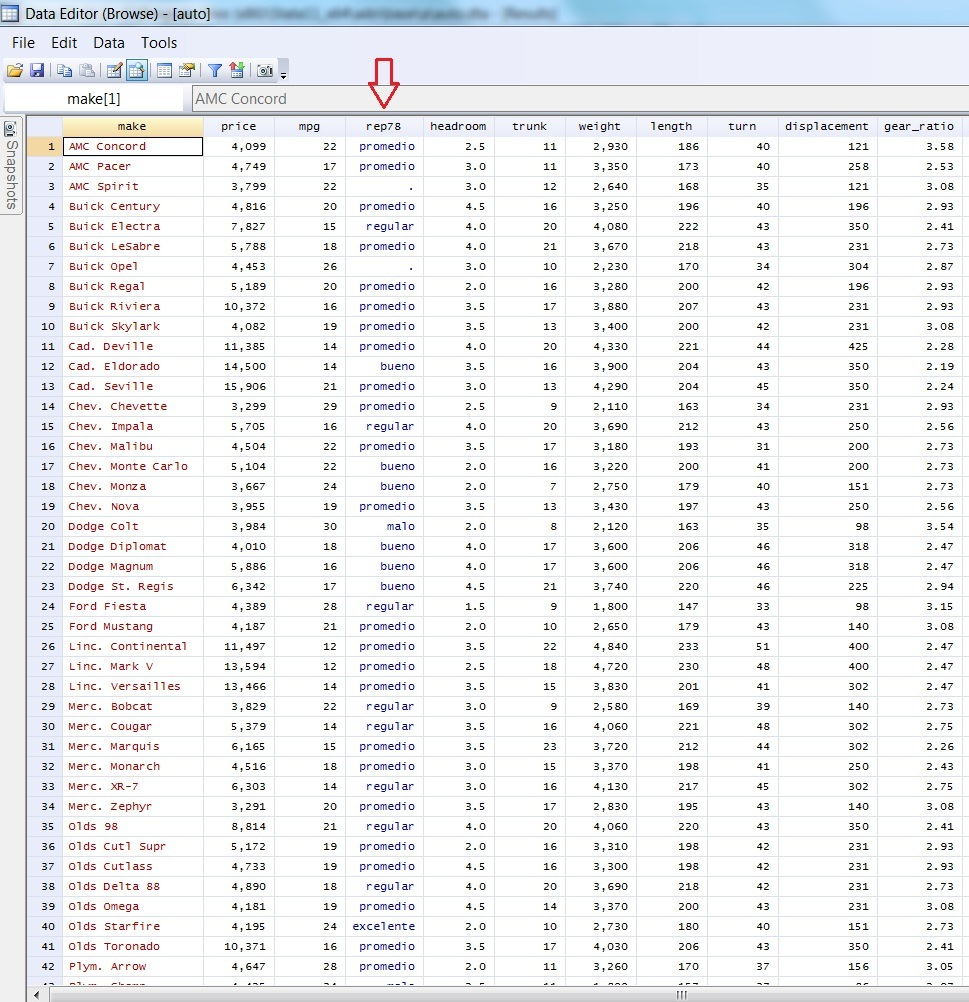
\includegraphics[height=6.5cm]{label1.jpg}}
\end{frame}


\begin{frame}{Summarize}
\begin{itemize}
\item El comando \texttt{summarize} nos presenta algunas estadísticas descriptivas de las variables: promedio, desvío estándar (DE), valores máximos y míminos. 
\item Así vemos por ejemplo que el precio promedio de los autos es $\$6.165,26$ y que el DE del peso es $\$777,2$.
\item En el caso de la variable "make", no numérica, no pueden calcularse estos estadísticos.
\end{itemize}
\centerline{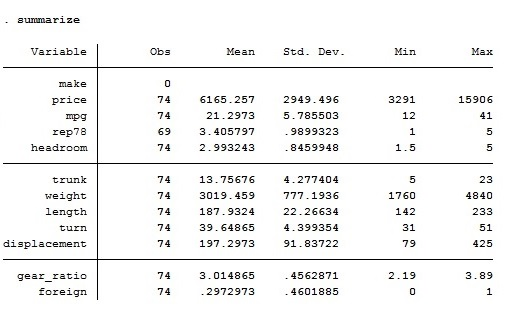
\includegraphics[height=3.3cm]{summerize.jpg}}
\end{frame}

\subsection{Summarize}

\begin{frame}{Summarize}
\begin{itemize}
\item El comando \texttt{summarize} podemos aplicarlo a toda la base o solo a alguna/s variable/s en particular.
\item También podemos hacer uso de la opción \texttt{detail} para acceder a estadísticos adicionales. 
\item Para ver más estadísticos de la variable ``price'' escribimos:
\centerline{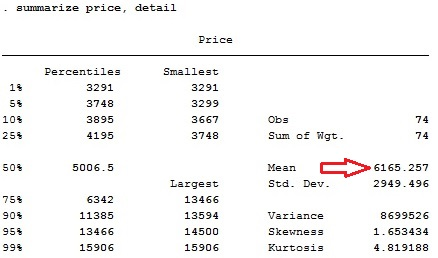
\includegraphics[height=3.5cm]{summarize1.jpg}}
\item Notar que \texttt{detail} se ha escrito después de una coma.
\end{itemize}
\end{frame}

\section{Tablas}
\begin{frame}{Tablas en STATA}
\begin{itemize}
\item En STATA existen varios comandos para producir tablas estadísticas. 
\item En esta clase veremos tres de los más importantes: \texttt{tabulate}, \texttt{tabstat} y \texttt{table}.
\item Si bien estos comandos se superponen en varias de sus funciones -el mismo resultado muchas veces puede obtenerse usando cualquiera de los tres- es importante apreciar sus diferencias y especificidades para utilizar el que mejor se adapte a nuestras necesidades en cada caso.
\end{itemize}
\end{frame}


\subsection{Tabulate}
\begin{frame}{Tabulate}
\begin{itemize}
\item El comando más sencillo es \texttt{tabulate}, que produce tablas de frecuencias (cantidad de observaciones para cada uno de los valores de una variable).
\item Por ejemplo, si escribimos \texttt{tabulate rep78} vemos que en la base hay 8 autos ($11,6\%$) que fueron reparados 2 veces.
\centerline{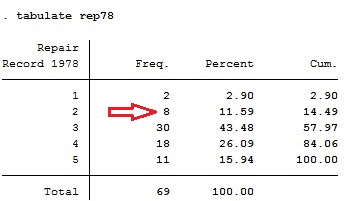
\includegraphics[height=3.2cm]{tabulate.jpg}}
\end{itemize}
\end{frame}


\begin{frame}{Tabulate}
\begin{itemize}
\item \texttt{tabulate} también nos permite cruzar dos variables, por ejemplo ``rep78'' y ``foreign'':
\centerline{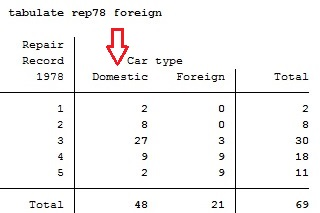
\includegraphics[height=3.5cm]{tabulate1.jpg}}
\item En columna señalada vemos por ejemplo cómo se distribuye la variable ``rep78'' para los autos domésticos.
\end{itemize}
\end{frame}

\begin{frame}{Tabulate}
\begin{itemize}
\item Quizás les llame la atención el hecho de que en la tabla anterior el total de observaciones era 69 y no 74, como habíamos visto que tenía la base. 
\item Esto es así porque hay 5 observaciones que no tienen ningún valor para la variable ``rep78''.
\item Estos casos se denominan \textit{missing}. 
\item Podemos hacer uso de la opción \texttt{missing} del comando \texttt{tabulate} para que nos muestre los valores faltantes (notar que se escribe después de una coma).
\end{itemize}
\end{frame}
\begin{frame}{Tabulate}
\centerline{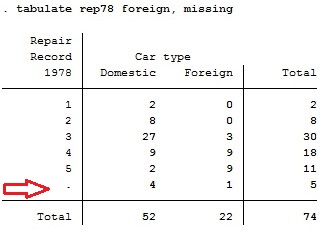
\includegraphics[height=4cm]{missing.jpg}}
\begin{itemize}
\item Como vimos, hay cinco observaciones \textit{missing} para ``rep78'', cuatro de los cuales corresponden a autos domésticos y uno a autos extranjeros.
\end{itemize}
\end{frame}



\subsection{Tabstat}

\begin{frame}[allowframebreaks]{Tabstat}
\begin{itemize}
\item \texttt{tabstat} presenta estadísticas descriptivas para variables numéricas:\\
\medskip
\centerline{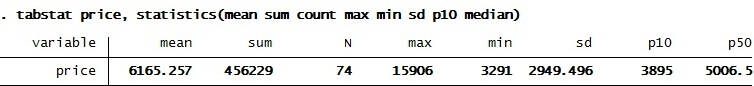
\includegraphics[height=1.2cm]{tabstat.jpg}}
\item Puede ser una buena alternativa al comando \texttt{summarize} porque permite especificar qué estadísticos queremos ver.
\item Podemos presentar más de una variable:\\
\medskip
\centerline{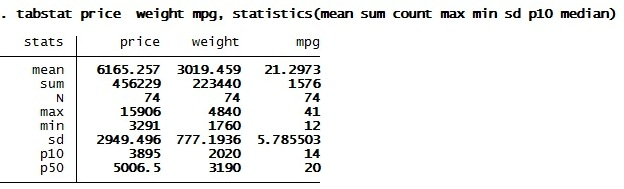
\includegraphics[height=2.2cm]{tabstat1.jpg}}
\item La opción \texttt{by()} nos permite presentar los estadísticos para las distintas categorías de otra varible:
\centerline{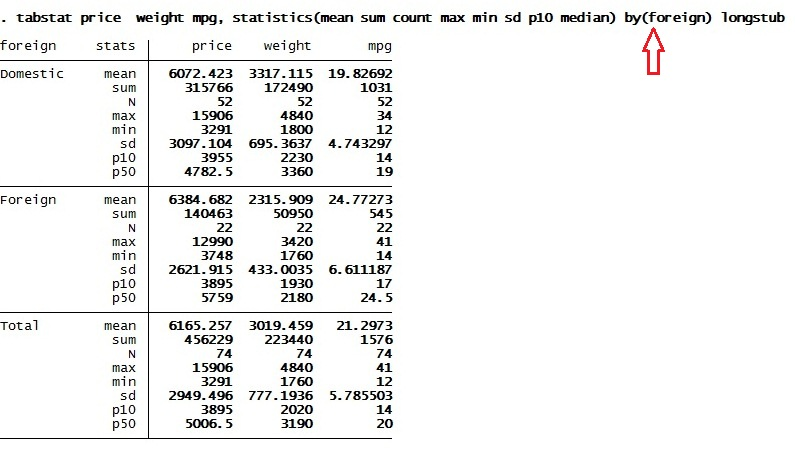
\includegraphics[height=5.2cm]{tabstat3.jpg}}
\item Después de la coma se utiliza la opción \texttt{statistics} y entre paréntesis se enumaran los estadísticos que se quieren calcular.
\item Se pueden calcular los siguientes estadísticos (entre otros): frecuencia (freq), promedio (mean), desvío estándar (sd), suma (sum), n (cant. de observaciones no missing), máximo (max), mínimo (min), mediana (median), pX (percentil $X$ -$X$ de cero a cien) y rango intercuartil (iqr). 
\end{itemize}
\end{frame}

\subsection{Table}
\begin{frame}[allowframebreaks]{Table}{Tablas de una entrada}
\begin{itemize}
\item \texttt{table} nos permite realizar tablas más complejas.
\item Por ejemplo, precio promedio de autos nacionales y extranjeros:
\medskip
\centerline{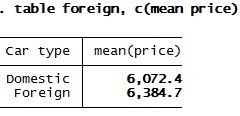
\includegraphics[height=1.7cm]{table.jpg}}
\item Podemos incluir más de un estadístico (hasta 5 columnas): 
\medskip
\centerline{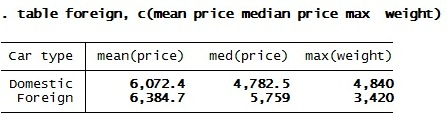
\includegraphics[height=1.7cm]{table4.jpg}}
\item En la tabla anterior vemos precio promedio, precio mediano y peso máximo del auto según origen. 
\item Para especificar el contenido de la celda escribimos primero el estadístico que queremos calcular y luego el nombre de la variable sobre la cual queremos calcularlo.
\item Se pueden calcular los siguientes estadísticos (entre otros): frecuencia (freq), promedio (mean), desvío estándar (sd), suma (sum), n (cant. de observaciones no missing), máximo (max), mínimo (min), mediana (median), pX (percentil $X$ -$X$ de cero a cien) y rango intercuartil (iqr). 
\end{itemize}
\end{frame}

\begin{frame}[allowframebreaks]{Table}{Tablas de doble entrada}
\begin{itemize}
\item Con \texttt{table} también podemos hacer tablas de doble entrada:
\centerline{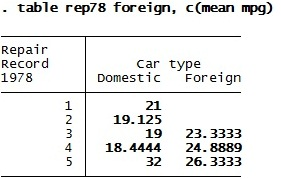
\includegraphics[height=2.5cm]{table5.jpg}}
\item En la tabla vemos el kilometraje promedio del auto por origen y cantidad de reparaciones.
\item Notar las celdas vacías: no existen esas combinaciones de origen y registro de reparaciones en nuestra base de datos.
\item Con \texttt{table} en las tablas de doble entrada también podemos incluir más de un estadístico:\\
\medskip
\centerline{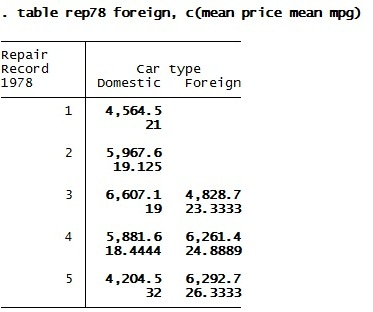
\includegraphics[height=3.9cm]{table6.jpg}}
\end{itemize}
\end{frame}

\section{Bibliografía y recursos Web}

\begin{frame}[allowframebreaks]{Bibliografía y recursos web}
Para complementar y profundizar los contenidos del curso se recomienda:
\begin{itemize}
\item Consultar la documentación oficial de STATA, en especial los manuales \textit{Getting Started} y \textit{User's Guide} (dentro del programa pueden ir a Help $>$PDF Documentation). 
\item Para profundizar sobre los conceptos estadísticos: Hamilton (2009), \textit{Statistics with STATA}. 
\item Para profundizar en las herramientas analíticas para el estudio de la pobreza y desigualdad (y su implementación en STATA) con aplicaciones a América Latina: Gasparini, L., M. Cicowiez y W. Sosa Escudero (2012), \textit{Pobreza y Desigualdad en América Latina: Conceptos, herramientas y aplicaciones}. 
\item Existen también varios tutoriales de STATA \textit{on line} que se pueden consultar:
\begin{itemize}
\item \url{www.cpc.unc.edu/research/tools/data_analysis/statatutorial}
\item \url{www.ats.ucla.edu/stat/stata}
\item \url{data.princeton.edu/stata/default.html}
\end{itemize}
\end{itemize}
\end{frame}



\end{document}

